\documentclass[11pt]{article}
\addtolength{\oddsidemargin}{-1.cm}
\addtolength{\textwidth}{2cm}
\addtolength{\topmargin}{-2cm}
\addtolength{\textheight}{3.5cm}
\newcommand\tab[1][1cm]{\hspace*{#1}}
\usepackage[pdftex]{graphicx}
\usepackage{pdflscape}
\usepackage[T1]{fontenc}
\usepackage{hyperref}
\usepackage{float}
\usepackage{cite}
\hypersetup{
	colorlinks=true,
	linkcolor=black,
	filecolor=magenta,
	urlcolor=cyan,
}

% define the title
\author{Binary Ninjaz}
\title{Harvest}
\begin{document}
\begin{titlepage}

	\begin{center}
		% Upper part of the page
		\textsc{\LARGE Binary Ninjaz}\\[0.3cm]
		% Title
		\rule{\linewidth}{0.5mm} \\[1cm]
		{ \huge \bfseries Harvest (User Manual)}\\[0.5cm]
		\rule{\linewidth}{0.5mm} \\[1cm]


		\begin{minipage}{0.4\textwidth}
			\begin{flushleft} \large
				\emph{} \\
				Letanyan {Arumugam}
			\end{flushleft}
		\end{minipage}
		\begin{minipage}{0.4\textwidth}
			\begin{flushright} \large
				\emph{} \\
				14228123
			\end{flushright}
		\end{minipage}

		\begin{minipage}{0.4\textwidth}
			\begin{flushleft} \large
            	\emph{} \\
				Sizo {Duma}
			\end{flushleft}
		\end{minipage}
		\begin{minipage}{0.4\textwidth}
			\begin{flushright} \large
				\emph{} \\
				15245579
			\end{flushright}
		\end{minipage}

		\begin{minipage}{0.4\textwidth}
			\begin{flushleft} \large
				\emph{} \\
				Teboho {Mokoena}
			\end{flushleft}
		\end{minipage}
		\begin{minipage}{0.4\textwidth}
			\begin{flushright} \large
				\emph{} \\
				14415888
			\end{flushright}
		\end{minipage}

		\begin{minipage}{0.4\textwidth}
			\begin{flushleft} \large
				\emph{} \\
				John {Ojo}
			\end{flushleft}
		\end{minipage}
		\begin{minipage}{0.4\textwidth}
			\begin{flushright} \large
				\emph{} \\
				15096794
			\end{flushright}
		\end{minipage}

        \begin{minipage}{0.4\textwidth}
			\begin{flushleft} \large
				\emph{} \\
				Kevin {Reid}
			\end{flushleft}
		\end{minipage}
		\begin{minipage}{0.4\textwidth}
			\begin{flushright} \large
				\emph{} \\
				15008739
			\end{flushright}
		\end{minipage}
        
        \begin{minipage}{0.4\textwidth}
			\begin{flushleft} \large
				\emph{} \\
				Shaun {Yates}
			\end{flushleft}
		\end{minipage}
		\begin{minipage}{0.4\textwidth}
			\begin{flushright} \large
				\emph{} \\
				16007493
			\end{flushright}
		\end{minipage}

		\vspace{0.5cm}
		\rule{\linewidth}{0.5mm} \\[1cm]
		\textsc{\Large Stakeholders}\\[1cm]

		\begin{minipage}{0.4\textwidth}
			\begin{flushleft} \large
				\emph{} \\
				SAMAC:
			\end{flushleft}
		\end{minipage}
		\begin{minipage}{0.4\textwidth}
			\begin{flushright} \large
				\emph{} \\
				Barry Christie
			\end{flushright}
		\end{minipage}


	\end{center}
\end{titlepage}

\newpage
\tableofcontents

\newpage
\section{General Information}
\subsection{System Overview}
Harvest, is an application to assist growers with yield data and optimise worker performance. In other words, it is a system that can efficiently measure the amount of work done by a worker, track the foremen on a farm, record information and data, and display the necessary information. This system is aimed at farming communities to help then record data and get work done more efficiently.\\

\subsection{System Requirments}
\subsubsection{Android}
The Android application currently requires:
\begin{itemize}
	\item Either Android 4.0 OS or above
\item 200 MB RAM
\item 50 MB Disk Space	
	\item Location Services
\end{itemize}
\subsubsection{iOS}
The iOS application currently requires:
\begin{itemize}
	\item iOS 10.0 or above
\item 200 MB RAM
\item 50 MB Disk Space	
	\item Location Services
\end{itemize}
\subsubsection{Website}
The website requires any modern up-to-date web browser such as Vivaldi, Firefox, Opera, Chrome, Safari, or any other.

\subsection{Networking}
All of the subsystems---Android, iOS, and website---run independintly, but use Firebase\footnote{\url{https://firebase.google.com}} to store and retrieve data from a common source.

\begin{figure}
 \centering
 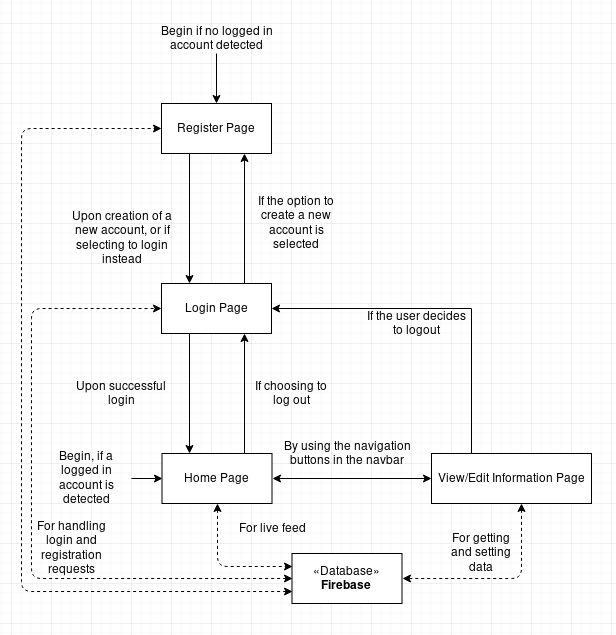
\includegraphics[width=12cm, keepaspectratio]{Images/Map.png}
 \caption{Website Map}
 \label{WebsiteMap}
\end{figure}

\subsection{Installation}
For Android devices the application will be available on the Google Play Store for download and for iOS devices the application will be available on the App Store.\\
With regards to configuration, location services are required. The user will be prompted for the location permissions in mention to allow full functionality of the application. Profile setting can be configured via selecting the user's username.\\

\newpage
\section{Getting Started}

\subsection{Creating an Account}
The application will open by default on the log in screen. If you do not have an account you can press the "Sign Up" button. Once on the sign up page enter your details an press "Create Account". You will then be logged in accordingly.

\subsection{Logging In}
When on the log in screen enter your email and its password you used to create the account. If you have already logged in the app will keep you logged in until you log out.

\subsection{Logging Out}
The Log out button can be found at the bottom of the Harvest "Settings" Tab.

\newpage
\section{Using the System}

\subsection{Using the Clicker}
When using the clicker ensure that you start the session first before clicking a worker to collect a yield from them. The procedure of using the clicker works as follows:

\begin{enumerate}
\item Press "Start"
\item Click a workers name when they bring in a bag.
\item Press "Stop"
\end{enumerate}

\newpage
\section{Troubleshooting}.

\subsection{Location Services}
\begin{enumerate}
\item Check that your phone supports location services
\item In the "Settings" application make sure that the Harvest app is allowed location services 
\end{enumerate}

\subsection{Forgotten Password}
\begin{enumerate}
\item On the sign in screen, tap "Forgot account details?" button.
\item When asked for your email, enter the the email address of the account with the forgotten password.
\item An email will be sent to that address.
\item Follow the instructions in the email. You will click on a link in the email.
\item From the web page that the link sent you to, Enter the new password for your account.
\item Log in to Harvest using your new details.
\end{enumerate}

\end{document}
